\section{Эксперимент и результаты}

Мы демонстрируем работу алгоритма, экспериментально факторизуя три целых числа
на сверхпроводящем квантовом процессоре, где выбраны десять кубитов и девять
соединителей, расположенных в топологии цепочки. Все кубиты и соединители — это
настраиваемые по частоте сверхпроводящие кубиты (transmon --- трансмон);
однокубитные вращения вокруг осей $x$ или $y$ сферы Блоха реализуются подачей
управляющих сигналов, в которых информация затвора закодирована в амплитуде и
фазе СВЧ‑импульсов. Виртуальные $z$‑затворы используются для выполнения
вращений вокруг оси $z$. Двухкубитные затворы с контролируемой файзой (CZ)
реализуются за счёт обмена совместными состояниями $|11\rangle$ и $|02\rangle$
(или $|20\rangle$) соседних кубитов, когда активируется взаимодействие,
передаваемое через соединитель \cite{cite_34}. Параллельные измерения
производительности кросс-энтропии (XEB --- cross-entropy benchmarking) дают
средние достоверности порядка $99{,}9\,\%$ для однокубитных вращений и
$99{,}5\,\%$ для CZ‑затворов. Подробности экспериментальной установки и
характеристики процессора приведены в \cite{cite_31}.

Мы факторизуем 11‑битное число $1961$, 26‑битное число $48567227$ и 48‑битное
число $261980999226229$, используя соответственно 3, 5 и 10 сверхпроводящих
кубитов. Ниже показан процесс получения одной sr‑пары квантовым методом в
каждой серии экспериментов. Вычисления остальных sr‑пар аналогичны и
выполняются численно; все sr‑пары и соответствующие системы линейных уравнений
приведены в \cite{cite_31}.

Топология $ZZ$‑слагаемых в гамильтониане задачи согласно уравнению (4)
представляет собой $K_n$ --- полный граф порядка $n$ \cite{cite_31}. Пример для
10 кубитов показан на рис. \ref{fig:fig02}B. Чтобы реализовать гамильтониан
типа $K_n$ на линейной 1D-цепочке физических кубитов, мы используем маршрутный
метод, основанный на классическом параллельном алгоритме пузырьковой
сортировки: все‑ко‑всем взаимодействия кубитов отображаются на взаимодействия
ближайших друг к другу двух кубитов с помощью cложных swap сетей, как показано
на рис. \ref{fig:fig02}D. Этот маршрутный метод является оптимальным и
добавляет лишь линейное увеличение глубины схемы. SWAP сети компилируются в
затворы рис. (рис. \ref{fig:fig02}E), которые могут исполняться непосредственно
на квантовом процессоре. Отметим маленький приём: чередование блоков ZZ‑SWAP
вверх‑вниз в чётных и нечётных слоях сетей позволяет сократить линейное число
затворов $H$.

\begin{figure}
    \centering
    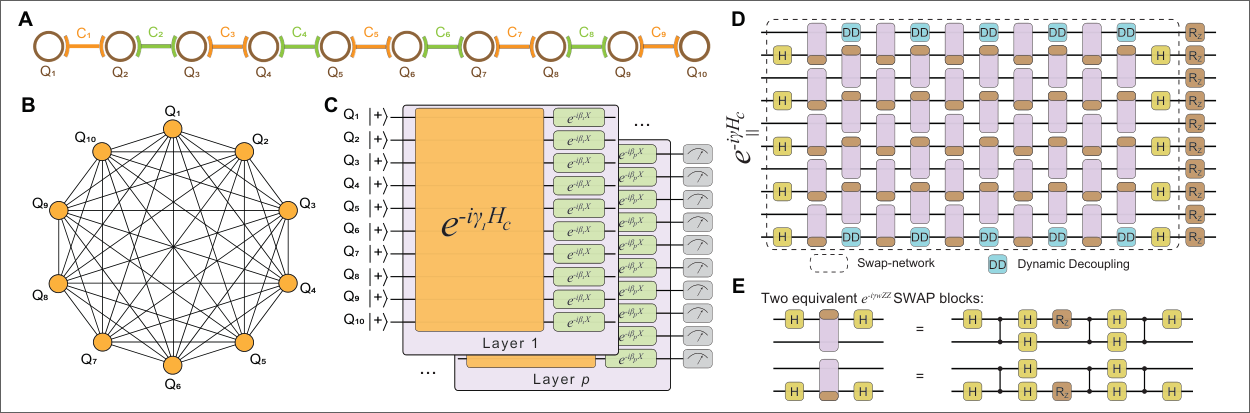
\includegraphics[scale=0.38]{inc/fig_02.png}
    \caption{
        Экспериментальная установка и схема QAOA алгоритма SQIF. \textbf{A}.
        Десять выбранных кубитов на сверхпроводящем квантовом процессоре;
        каждый кубит связан с ближайшими соседями через настраиваемые по
        частоте соединители. \textbf{B}. Родная топология взаимодействий
        гамильтониана задачи для случая факторизации на 10 кубитах,
        отображённая в линейную цепочку, показанную в A. \textbf{C}. Схема
        $p$‑слойного QAOA. Все кубиты инициализируются в состояние $|+\rangle$,
        далее следуют $p$ слоёв попеременного действия гамильтониана задачи
        (оранжевый) и смешивающего гамильтониана (зелёный) и завершающие
        измерения популяций (серый). Обратите внимание, что вариационные
        параметры $\{\gamma,\beta\}$ различны для каждого слоя. \textbf{D}.
        Маршрутная схема для отображения все‑к‑о‑всем гамильтониана 10 кубитов
        на линейную топологию ближайших соседей; построена «кирпичной» сеткой
        из двух одинаковых блоков SWAP с двумя слоями затворов $H$ (Hadamard) в
        начале и конце, за которыми следует слой затворов $R_z(\theta)$. Здесь
        угол вращения опущен. Глубина схемы пропорциональна числу
        задействованных кубитов. \textbf{E}. Подробная компиляция квантовой
        схемы в затворы сверхпроводящего квантового процессора.
    }
    \label{fig:fig02}
\end{figure}

QAOA находит приближённое основное состояние гамильтониана путём обновления
параметров (рис. \ref{fig:fig02}C; подробности см. \cite{cite_31}). Оптимизацию
параметров QAOA можно проиллюстрировать через ландшафт функции энергии
$E(\gamma,\beta)$. Сравнение теоретического и экспериментального ландшафтов
служит качественной диагностикой применимости QAOA на реальном оборудовании.
Для гиперпараметра $p=1$ ландшафт энергии как функция $(\gamma,\beta)$
изображён в 3D графике на рис. \ref{fig:fig03}. Значения энергии нормированы по
$E^{\ast}=(E-E_{\min})/(E_{\max}-E_{\min})$. На рис. \ref{fig:fig03} показаны
симуляция без шума (слева) и эксперимент (справа) для случаев 3, 5
и 10 кубитов. Различные цвета пикселей обозначают разные значения функции;
поверх наложена траектория сходимости классического оптимизатора (красная
кривая). Для оптимизации используется метод градиентного спуска по модели,
показавший хорошую работу как в теории, так и на практике. Алгоритм сходится в
область глобального минимума менее чем за 10 шагов во всех трёх случаях. Хотя
пути сходимости эксперимента отличаются от теоретических, они достигают
оптимума за сравнимое число шагов. Это свидетельствует об устойчивости
алгоритма к определённому уровню шума.

\begin{figure}
    \centering
    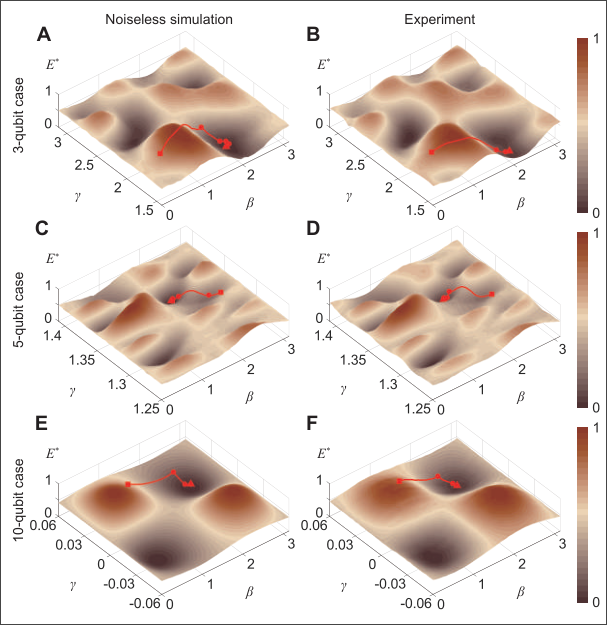
\includegraphics[scale=0.4]{inc/fig_03.png}
    \caption{
        Энергетические ландшафты и траектории сходимости QAOA при $p = 1$.
        \textbf{A}, \textbf{B} — численные и экспериментальные ландшафты для
        случая 3 кубитов; \textbf{C}, \textbf{D} — для 5 кубитов; \textbf{E},
        \textbf{F} — для 10 кубитов. В каждой экспериментальной группе оценены
        $41\times 41$ комбинаций $(\gamma,\beta)$, равномерно распределённых по
        сетке в подобласти всего двумерного пространства параметров. Для каждой
        точки сетки математическое ожидание энергии вычисляется по результатам
        $30\,000$ повторов схемы. Сравнение экспериментальных и численных
        ландшафтов демонстрирует отчётливое соответствие характерных
        особенностей. Наложенная траектория оптимизации (красная; стартует из
        квадратного маркера и сходится в треугольник) показывает способность
        классического оптимизатора находить оптимальные параметры.
    }
    \label{fig:fig03}
\end{figure}

В QAOA основная работа квантового компьютера состоит в подготовке квантовых
состояний с заданными вариационными параметрами. Теоретически
производительность QAOA улучшается с ростом глубины гиперпараметра $p$. Однако
с увеличением глубины накапливаются ошибки, и выгода может нивелироваться. Ниже
приведены результаты процессора при оптимальных $(\beta,\gamma)$. Мы
демонстрируем слои QAOA до $p=3$ для 3‑ и 5‑кубитных случаев и односоставную
QAOA ($p=1$) для 10 кубитов. Для 10 кубитов также выполнен запуск при $p=3$;
результат лучше случайного угадывания, но хуже, чем при $p=1$ \cite{cite_31}.
На рис. \ref{fig:fig04}A‑C видно, что вероятность целевого состояния (красная
пунктирная рамка) растёт с увеличением $p$. Хотя рост меньше теоретического, он
хорошо согласуется с шумовой симуляцией. Аналогичные результаты получены в
5‑кубитном эксперименте (рис. \ref{fig:fig04}D‑F). Для 10 кубитов при $p=1$
результаты показаны на рис. \ref{fig:fig04}G; для наглядности отображены 120
наиболее вероятных состояний по теории. Теоретическая вероятность целевого
состояния равна 0.02 (наибольшая), экспериментальная около 0.008, что близко к
шумовому значению 0.009. Экспериментальные результаты значительно превосходят
случайное угадывание 0.001, то есть вычислительный выигрыш QAOA остаётся
существенным. Более того, форма распределения вероятностей симметрична
относительно симуляционных данных, что также подтверждает хорошее совпадение
эксперимента с теорией.

\begin{figure}
    \centering
    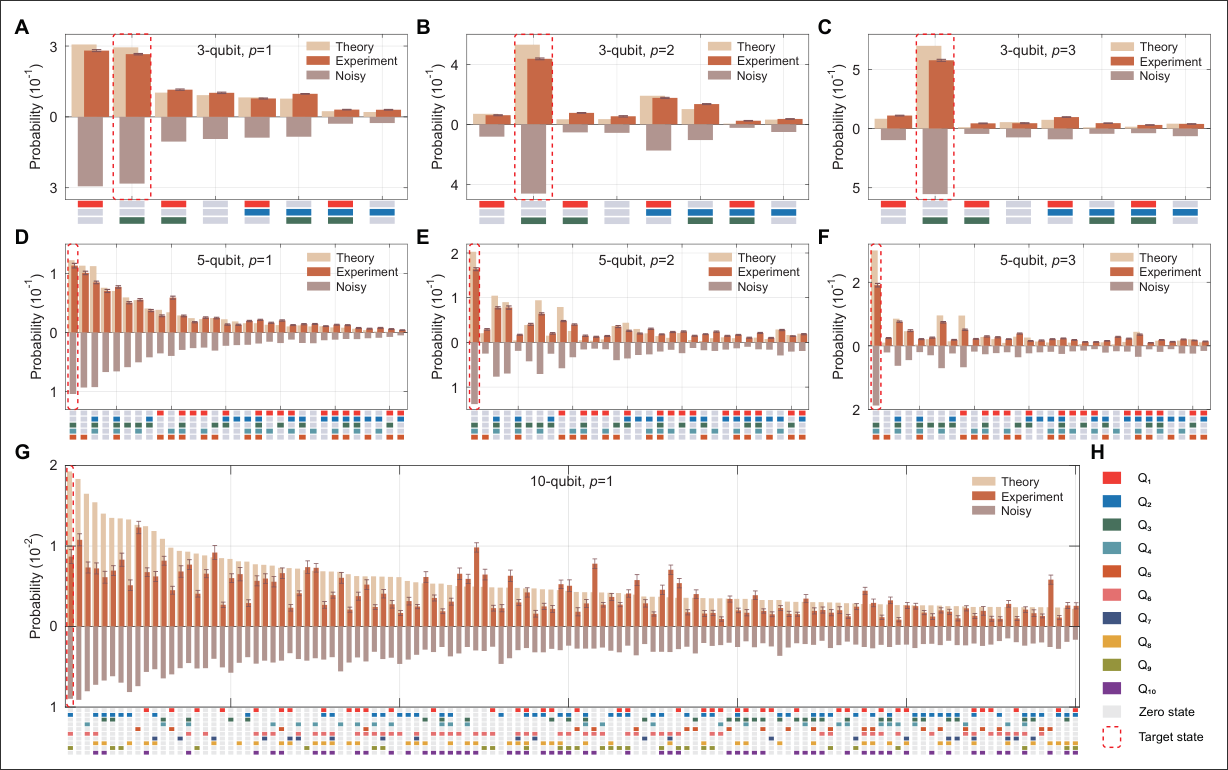
\includegraphics[scale=0.38]{inc/fig_04.png}
    \caption{
        Экспериментальная производительность QAOA для трёх случаев
        факторизации. \textbf{A–C}. Производительность QAOA для 3‑кубитного
        случая при $p = 1$, $p = 2$ и $p = 3$ соответственно. \textbf{D–F}.
        Производительность QAOA для 5‑кубитного случая при $p = 1$, $p = 2$
        и $p = 3$ соответственно. \textbf{G}. Производительность QAOA при $p =
        1$ для 10‑кубитного случая. Экспериментальные результаты, показанные
        оранжевым цветом, усреднены по 20 повторам эксперимента; штрихи ошибок
        отображают доверительный интервал в одном стандартном отклонении. Для
        сравнения также приведены теоретические (жёлтый) и шумовые при
        уровне 0.01 (серо‑тауповый) результаты. Видно, что все три группы
        экспериментальных данных на сверхпроводящем квантовом процессоре хорошо
        согласуются с теорией и шумовой моделью 0.01. \textbf{H}. Обозначения
        цветовых блоков, соответствующих базисным состояниям различных кубитов
        в подписи оси $x$.
    }
    \label{fig:fig04}
\end{figure}

